\chapter{Literature Survey}
\label{chapter:literature} 
\noindent\rule{\linewidth}{2pt}

\section{Introduction}
Artificial Intelligence has been used in medical sciences for a long time and have advanced significantly. However, the introduction of AI in retinal diseases is quite recent. This chapter gives a summary of the recent works that have been carried out in this area. OCT is an interferometric scanning method which captures cross-sectional view of the biological tissues. It uses light’s coherent properties which have not been widely used previously in methods involving medical sciences.

\section{Study of Optical Coherence Tomography in Recent Publications}
Schmitt \cite{Schmitt} focused on the development of early OCT imaging methods and its introduction to the medical sciences. OCT provides a better structural and detailed view of the different sections of the eye as compared to confocal and bright field microscopes. The applications of OCT in ophthalmology have been recorded for the first time by Osiac et al. \cite{Osiac2011} and studied by Ţălu and Ţălu\cite{simonaDelia} in their research work. The authors focused specifically on AMD, providing a better insight into how OCT images are helpful for the identification of the diseases, the TD-OCT, and its progress to SD-OCT. Schmidt-Erfurth et al. \cite{Schmidt2017} explored and studied the use of OCT in monitoring and detection of AMD and early signs of AMD, Drusen and identify the progression of the diseases. The works of both the papers provided an analysis on why SD-OCT has been widely used for diagnosis, which provides a volumetric and cross-sectional view as compared to TD-OCT which gives only the cross-sectional view, i.e., a 2D perspective of the retina.

\section{Methodologies and Procedures Employed in Recent Publications}
A classification approach was published by Srinivasan et al. \cite{Srinivasan2014} based on Support Vector Machine \cite{708428} (SVM) which used multi-scale histograms as feature vectors to classify OCT images into AMD, DME and normal eyes. The work uses Block-matching and 3D Filtering \cite{6086619} (BM3D) for noise removal from SD-OCT images followed by resizing to a shape of 248 x 256. The retinal curvature of the image is flattened to approximate the curvature of all the images, as the curvature of each scan varies from patient to patient. The image is further cropped to 150 x 150 for feature extraction. The proposed method uses Support Vector Machine (SVM) for classification into multiple classes. It achieved high accuracy in detecting 100\% DME, 100\% AMD and 86.67\% of Normal eye images. Figure \ref{fig:Srinivasan2014} illustrates the process progression of the provided methodology.


\begin{figure}[htb]
\centering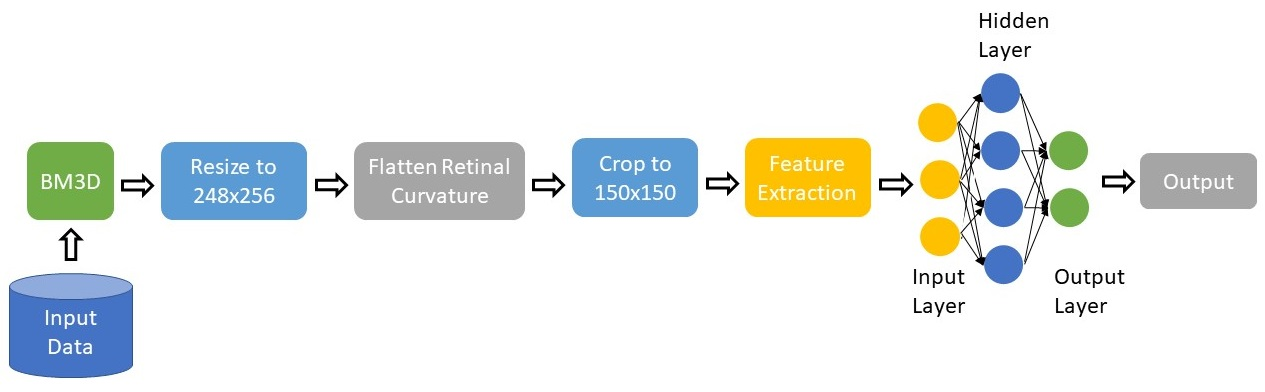
\includegraphics[width=\linewidth]{figimages/bm3dbased.jpg}
\caption{Process Flow of SVM based Classification Method proposed in \cite{Srinivasan2014}} 
\label{fig:Srinivasan2014}
\end{figure}

\par
Lemaître et al. \cite{Guillaume} focused on the classification of Diabetic Macular Edema (DME), amond the primary reasons of permanent vision loss in patients with diabetes. The OCT image data is de-noised using non-local means (NLM) filtering method, followed by flattening of the image curvature, like the flattening method used in the previous work. Further, the method uses feature extraction with five classical machine learning algorithms: k-NN, Logistic Regression, SVM, Random Forest, and Gradient Boosting for binary classification task. SERI dataset is used in the research work. For validation, specificity, sensitivity, confusion matrix, etc. parameters are visualized and assessed. Figure \ref{fig:Guillaume} visualizes all the steps of the given method.

\begin{figure}[htb]
\centering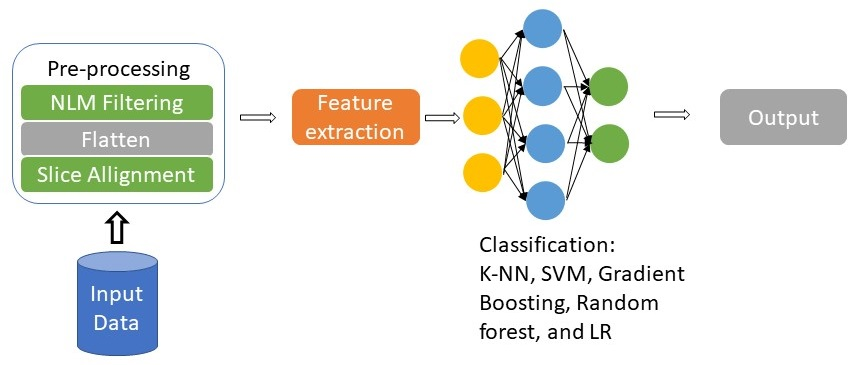
\includegraphics[width=\linewidth]{figimages/nlm6.jpg}
\caption{Classification Method proposed in \cite{Guillaume}} 
\label{fig:Guillaume}
\end{figure}

\par
Karri et al. \cite{Karri2017} introduced transfer learning approach for OCT-based classification of dieases in 3 classes, AMD, DME, and normal eye. The method uses pre-trained GoogleNet architecture for classification. The pre-processing phase consists of saturation removal, flattening followed by denoising. The pre-processed images are denoised using BM3D, followed by layer segmentation. The 3-channel input images fed to the GoogleNet are of dimensions 224x224. The Duke OCT dataset was used for training the said model and to evaluate the performance. The highest accuracy achieved was 96\%. This method proved that fine-tuned CNNs can be used to classify retinal pathologies effectively.

\begin{figure}[htb]
\centering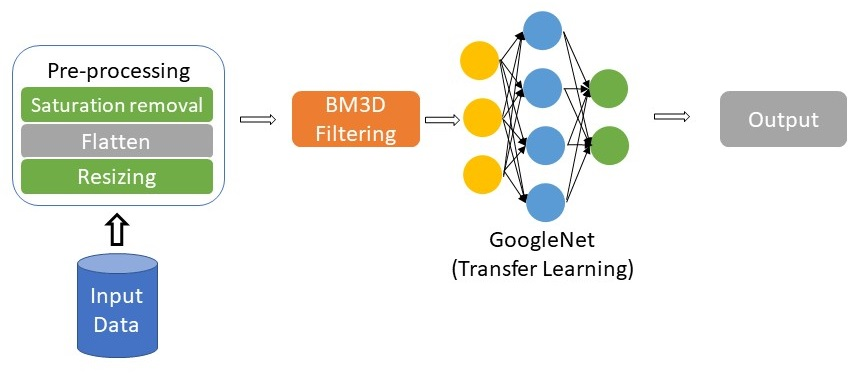
\includegraphics[width=\linewidth]{figimages/GoogleNet.jpg}
\caption{GoogleNet based method proposed in \cite{Karri2017}} 
\label{fig:Karri2017}
\end{figure}

\par
A binary classification method was given by Alsaih et al. \cite{Alsaih2017} for the detection of DME disease from SD-OCT images. The dataset was taken from SERI, Singapore consisting of 4,096 OCT images with normal and DME classes in ratio of 1:1. They diversified the data by selecting distinct lesions, i.e., abnormal tissue region in the Diabetic Macular Edema (DME) data sub-set. The proposed method used Principal Component Analysis \cite{WOLD198737} (PCA) in the classification pipeline with SVM resulting in a specificity of 87.5 and sensitivity of 87.5\%.

\par
Choi et al. \cite{Choi2017} used fundus photograph dataset of human eye from the publicly available dataset from Structured Analysis of the Retina (STARE) project for the CNN-based classification. MatConvNet \cite{VedaldiL14} architecture was used for the classification of retinal diseases. The dataset consisted of total of 10 classes including the normal human eye scans with each class containing around 1000 images each. The classification results were also obtained by using transfer learning method, specifically VGG19 architecture. Accuracy, RCI, and Kappa value were the parameters used for model evaluation. As the number of classes were increased to 10, the accuracy diminished to a low of 30.5\% on MatConvNet and a slightly better accuracy of 36.7\% on transfer learning method with VGG19 architecture. The process flow is described in Figure \ref{fig:Choi2017}.

\begin{figure}[htb]
\centering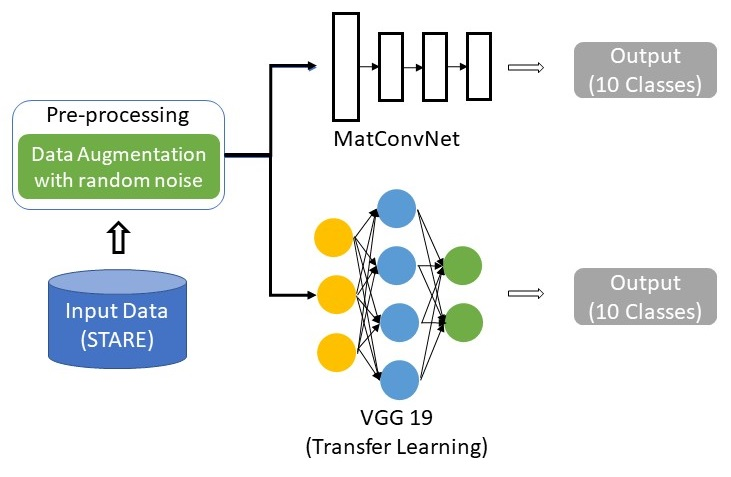
\includegraphics[width=\linewidth]{figimages/MatConvNet.jpg}
\caption{MatConvNet and VGG19 Classifier proposed in \cite{Choi2017}} 
\label{fig:Choi2017}
\end{figure}
\pagebreak
\par
In 2018, a novel method for classification of SD-OCT images of AMD, and DME was proposed by Hussain et al. \cite{Hussain2018}. The dataset consisted of 1,183 images of dimension 512x1024. The method involved segmentation of images for feature extraction and classification using various machine learning algorithms like SVM, Decision Tree, Random Forest out of which RF gave the best accuracy of 95\%. The proposed method can be visualized as below:

\begin{figure}[htb]
\centering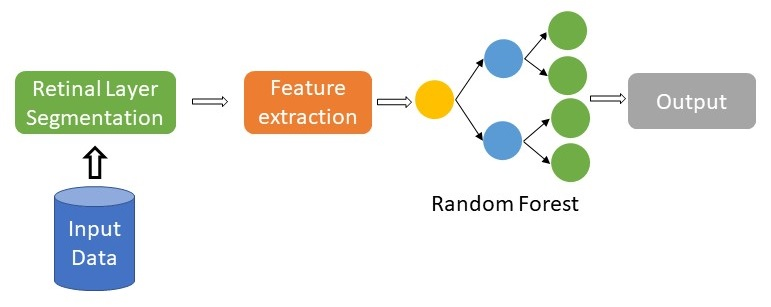
\includegraphics[width=\linewidth]{figimages/RandomForest.jpg}
\caption{Machine Learning based Classification of AMD and DME diseases} 
\label{fig:Hussain2018}
\end{figure}

\par
The research work proposed by Maetschke et al. \cite{Maetschke2019} involves a deep learning classification technique on unsegmented raw OCT scans, unlike its previous counterparts which used segmentation on OCT images before classification. The data includes scans from 624 patients having a total 1,110 images of healthy eye and 847 images of patients with Primary Open Angle Glaucoma (POAG). The images had a dimension of 200x1024. The evaluation metric used in this work was Area under the Receiver Operator Characteristic (AUC) curve. The proposed method classified a healthy eye with glaucomatous eyes using 3D CNN classifier with an accuracy of 94\%. This study proves that CNN can provide a good classification accuracy over raw unsegmented images in comparison to classical machine learning algorithms like k-NN, SVM, etc. The novel CNN architecture proposed in the above method consists of five 3D convolutional layers and a fully-connected layer. The architecture is described in the Figure \ref{fig:Maetschke2019}.

\begin{figure}[htb]
\centering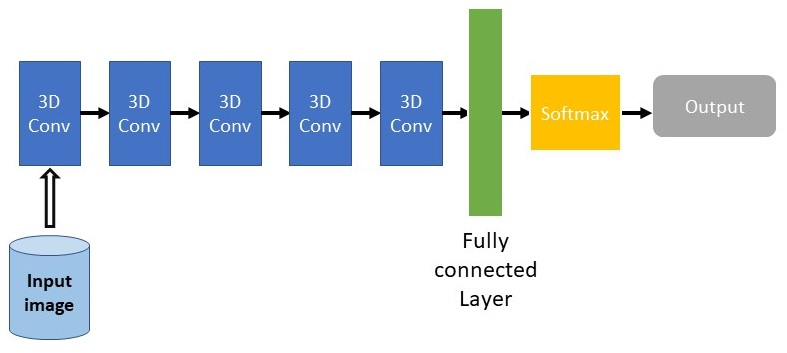
\includegraphics[width=\linewidth]{figimages/3DCNN.jpg}
\caption{3D CNN Architecture proposed in \cite{Maetschke2019}} 
\label{fig:Maetschke2019}
\end{figure}

\par
It is hard to automate the stacking of OCT images with a blurred layered structure and poor contrast.. Xiaoming et al. \cite{Xiaoming2019} resolved the issue by developing a novel OCT technique for detection that utilized complex Shearlet transforms. The evaluation data comprised of OCT images of Stargardt disease, dry AMD, and normal retinal macular region. The findings demonstrated that the complex Shearlet transform approach had been beneficial as it enabled the detection of more OCT image layers.

\par
Li et al. \cite{Li2019} devised and approach for classification of four ocular diseases including DME, CNV, Drusen and normal eye. The data was collected from Shanghai First People’s Hospital and Shanghai Zhongshan Hospital consisting of a total 15,573 OCT images, 3,786 in CNV, 3,238 in DME, 2,113 in Drusen, and 6,436 in normal eye. The evaluation parameters used in this method were accuracy, AUC curve, Kappa value, specificity, and sensitivity. The proposed method was based on transfer learning which employed a combination of 4 classification models which were formed using ResNet50 architecture, as shown in Figure \ref{fig:Li2019}, achieved an accuracy of 97.3\%.
\begin{figure}[htb]
\centering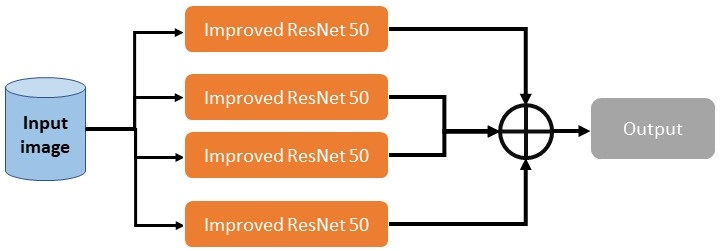
\includegraphics[width=\linewidth]{figimages/ResNet50.jpg}
\caption{ResNet50 Ensemble Classification Method \cite{Li2019}} 
\label{fig:Li2019}
\end{figure}

\par
One of the most recent and effective studies in the area of Retinal disease detection using SD-OCT images was carried out by Tayal et. al. \cite{Tayal2022}. The authors proposed three novel CNN architectures for the classification of DME, Drusen, CNV and normal eyes. The dataset used in this approach was taken from Mendeley Database having total 83,484 images. The images were then resized to 150x150 size and cropped to 128x128, where 128x128 being the input size for the CNN networks. The images were processed for noise removal using mean blur filter, contrast adjusted using Contrast Limited Adaptive Histogram Equalization (CLAHE) algorithm \cite{Sheet2022}, and edges were refined by drawing contours over them. The proposed method used 5-layered, 7-layered, and 9-layered convolutional neural networks which provided the highest accuracy of 96.5\%. This method's process flow is described in Figure \ref{fig:Tayal2022}.

\begin{figure}[htb]
\centering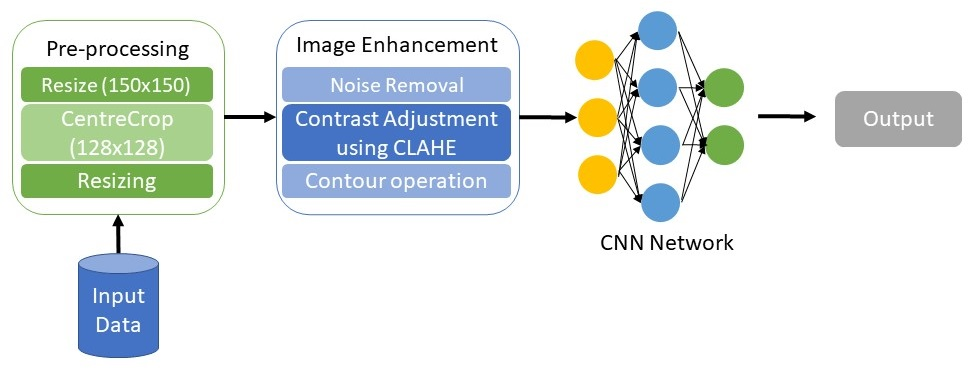
\includegraphics[width=\linewidth]{figimages/BasePaper.jpg}
\caption{Novel CNN architecture-based Classification method proposed in \cite{Tayal2022}} 
\label{fig:Tayal2022}
\end{figure}

\section{Problem Statement}
In accordance with World Health Organization (WHO) globally over 2.2 billion people have visual impairment out of which 1 billion cases could have been prevented if diagnosed early. In the modern world, it is essential to address this problem by devise ways for easy and error free detection of retinal or ocular diseases for diagnosis and treatment. 

\par
The increasing availability of medical data, combined with advancements in artificial intelligence (AI) technology, has led to the exploration of AI-based disease classification in medical sciences. In the present world, the use of advancing technology and application of Computer Science and Artificial Intelligence is growing drastically, especially in the biomedical sector for various purposes such as medical treatment, disease detection and diagnosis, etc. Artificial Intelligence has helped in reducing time consumed in diagnosis along with minimizing the scope of human errors. A sub-section of all the applications of Artificial Intelligence in Biomedical science is in Medical Image processing and disease diagnosis, i.e., the classification of diseases with minimal error, utilizing various image processing techniques and classification techniques. The scope of AI in ocular disease classification has increased significantly with advancements in eye-imaging techniques and artificial intelligence making it useful for ophthalmologists to devise a better way of determining the probability of a disease and to provide an immediate treatment. 

\section{Objectives}
To devise an improved approach for the classification of retinal diseases using OCT scans, we propose the following objectives which will be achieved in this dissertation work:
\begin{itemize}
    \item To identify and classify the OCT images into five categories including four retinal diseases- AMD, Drusen, Macular Hole, CSR, and normal human eye.
    \item Introduce a deep learning-based noise removal technique for denoising OCT images to remove speckle noise, which in turn will improve the model performance.
    \item Develop a novel deep learning architecture for the multi-classification problem.
    \item Measure the various evaluation parameters of the trained model like confusion matrix, accuracy, precision, recall, etc.
\end{itemize}